\documentclass[english]{article}

\usepackage[english]{babel}
\usepackage{graphicx}
\usepackage{framed}
\usepackage[normalem]{ulem}
\usepackage{amsmath}
\usepackage{amsthm}
\usepackage{amssymb}
\usepackage{amsfonts}
\usepackage{enumerate}
\usepackage{fancyhdr}
\usepackage{parskip}

\usepackage{listings}
\usepackage[numbered,framed]{matlab-prettifier}


\lstset{
  style              = Matlab-editor,
  basicstyle         = \mlttfamily,
  escapechar         = ",
  mlshowsectionrules = true,
}

\usepackage[shortlabels]{enumitem}
\usepackage[nobreak=true]{mdframed}
\usepackage[left=0.75in,right=0.75in,top=0.75in,bottom=0.75in]{geometry}
\usepackage{hyperref}
\usepackage{epigraph}
\usepackage{setspace} 

\usepackage{amsmath,amsthm,amssymb} 

\usepackage{stmaryrd}  
\usepackage{ dsfont }
\usepackage{natbib} 

\usepackage{comment}

\usepackage{hyperref}

\usepackage{ulem}
\usepackage{gensymb}
\usepackage{mathrsfs}
\usepackage{mathtools}
\usepackage{fancyhdr}
\usepackage[nobreak=true]{mdframed}


\usepackage[T1]{fontenc}
\usepackage[utf8]{inputenc}


\hypersetup{colorlinks=true, citecolor=false, linkcolor=blue}  

\newcommand\tab[1][.5cm]{\hspace*{#1}}

\newcommand{\solution}[1]{
\textbf{Answers:\\}
{#1}
}

\newcommand{\subq}[1]{
\textbf{({#1}):\\}
}

\newcommand{\integral}[4]{
\int_{{#1}}^{{#2}} {#3} \text{ } {#4}
}

\newcommand{\norm}[2]{
||#1||_{#2}
}

\renewcommand{\thesubsection}{\thesection.\alph{subsection}}


\theoremstyle{definition}
\newtheorem{theorem}{Theorem}[section]
\newtheorem{observation}[theorem]{Observation}
\newtheorem{proposition}[theorem]{Proposition}
\newtheorem{corollary}[theorem]{Corollary}
\newtheorem{definition}[theorem]{Definition}
\newtheorem{keydefinition}[theorem]{Definition}
\newtheorem{lemma}[theorem]{Lemma}
\newtheorem{fact}[theorem]{Fact}
\newtheorem{example}[theorem]{Example}
\newtheorem{notation}[theorem]{Notation}
\newtheorem{remark}[theorem]{Remark}  
\newtheorem{problem}{Problem}  


\setcounter{secnumdepth}{0}

\newcommand{\yourName}{Josephine Odusanya}
\newcommand{\yourNetID}{joo9964}

\begin{document} 
\rfoot{Name: \yourName, netID: \yourNetID}
\title{\textbf{[Fall 2025] ROB-GY 6203 Robot Perception Homework 1}}
\author{\yourName}
\pagestyle{fancy}
\date{Submission Deadline (No late submission): NYC Time 5:00 PM, October 09, 2025}

\maketitle
\textbf{General Rules}

\begin{enumerate}
    \item Please submit the \textbf{.pdf} generated by this LaTex file. This .pdf file will be the main document for us to grade your homework. If you wrote any code, please zip all the \textbf{code} together and \textbf{submit a single .zip file}. Name the code scripts clearly or/and make explicit reference in your written answers. Do NOT submit very large data files along with your code!
    \item This Overleaf project is view-only. To work on this document, please use the download feature on the top left and download the source files. Then, you can re-upload them to your own Overleaf account or any other LaTeX editing tools of your preference.
    \item Please typeset your report in LaTeX/Overleaf. If you have never used LaTeX/Overleaf before, the best advice is to just start typing. Try things hands-on like a true engineer! If you prefer a more structured introduction, \hyperlink{https://www.youtube.com/watch?v=ydOTMQC7np0}{this video} can be a good help. \textbf{Do NOT submit a hand-written report!} as they will be graded zero. 
    
    LaTeX is the standard tool for STEM academic writing due to its convenience in typesetting mathematical formulas, so this class will encourage you to get familiar with this widely used tool.
    \item Do not forget to update the variables ``yourName'' and ``yourNetID''.
\end{enumerate}


\textbf{Hints}
\begin{enumerate}
    \item While the HW may talk about AprilTag, you don't have to use it. You can use similar, but more accessible options, such as OpenCV's ArUco tag.
    \item You don't have to print out a tag physically. Displaying them on a screen, such as your phone or iPad, would work most of the time. Make sure the background of the tag is white. In my experience, a tag on a black background is harder to detect.
\end{enumerate}

\tableofcontents
\clearpage

\section{Task 1 Sherlock’s Message (2pt)}
Detective Sherlock left a message for his assistant, Dr. Watson, while tracking his arch-enemy, Professor Moriarty. Could you help Dr. Watson decode this message? The original image itself can be found in the data folder of the Overleaf project, named \texttt{for\_watson.png}
\begin{figure*}[h!]
    \centering
    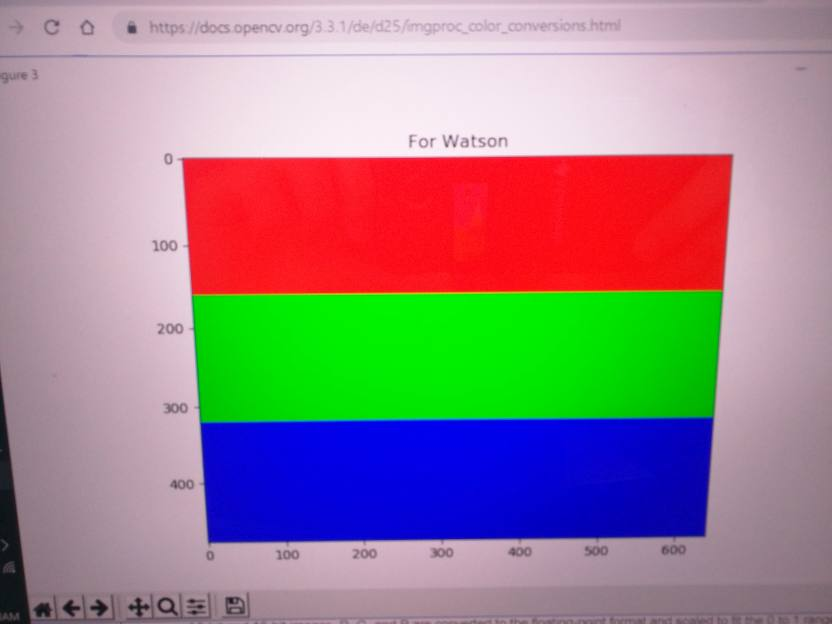
\includegraphics[scale = 0.4]{figs/screenshot.png}

    \caption{The Secret Message Left by Detective Sherlock}
    \label{fig:for_watson}
\end{figure*}\\

\subsection{a) (1pt)}
Please submit the image(s) after decoding. The image(s) should have the secret message on it(them). Screenshots or images saved by OpenCV is fine.

\solution{

You can use this code snippet to include a picture
\begin{figure}[h!]
    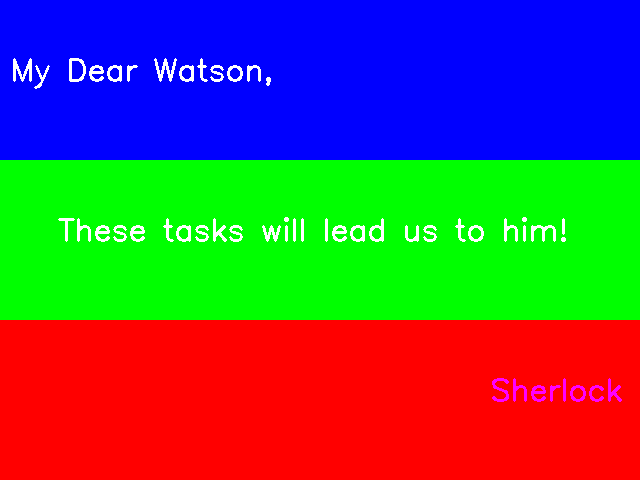
\includegraphics[scale = 0.3]{figs/task1_decoded_message.png}

    \label{fig:answer to task 1a}
\end{figure}

}

=======edit here

\subsection{b) (1pt)}
Please describe what you did with the image with words, and tell us where to find the code you wrote for this question.

\solution{
I had to play around with the function cv2.threshold, at first the image only showed the middle statement 
"these task will lead us to him". Then I changed the colour code to white (255) and black (0) to get the full message.
You can find the code to all 4 tasks here: \hyperlink{https://github.com/josephineoe/Robot-Perception/blob/main/Homework/homework1.ipynb}{here} \textbf

}

\clearpage



\section{Task 2. Low Dimensional Projection (5pt)}
Given the \href{https://github.com/zalandoresearch/fashion-mnist}{Fasion-MNIST dataset}, \textbf{train} an unsupervised learning neural network that gives you a lower-dimensional representation of the images, after which you could easily use tSNE from \texttt{Scikit-Learn} to bring the dimension down to 2. \textbf{Visualize} the results of all 10000 images in one single visualization.

\solution{

\begin{figure}[h!]
    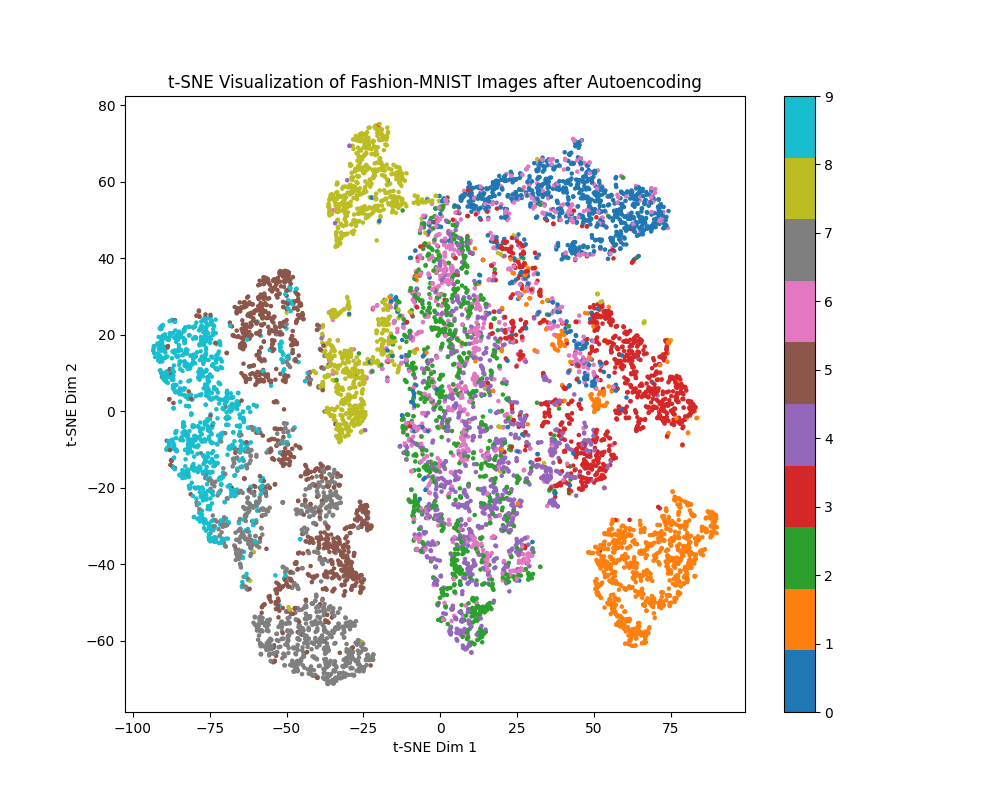
\includegraphics[scale = 0.3]{figs/task2_plot.png}

    \label{fig:answer to task 2}
\end{figure}

}

\clearpage

\section{Task 3 Camera Calibration (3pt)}

Use the pyAprilTag package provided in the class, or other free packages (e.g., OpenCV’s camera calibration toolkit) that you may be aware of, to \textbf{calibrate} your camera and provide the full K matrix, with the top two distortion parameters k1 and k2.

\solution{

\begin{figure}[h!]
    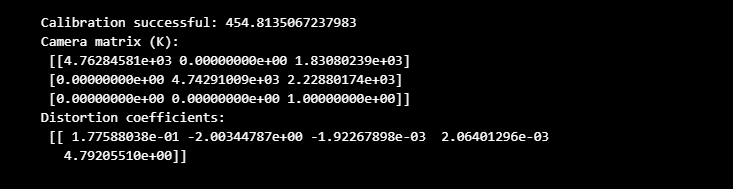
\includegraphics[scale = 0.3]{figs/task3_calib_results.png}

    \label{fig:answer to task 3 k matrix and distortion}
\end{figure}

}

\clearpage

\section{Task 4 Tag-based Augmented Reality (5pt)}
Use the pyAprilTag package to detect an AprilTag in an image (or use OpenCV for an Aruco Tag), for which you should take a photo of a tag. Use the K matrix you obtained above, to draw a 3D cube of the same size of the tag on the image, as if this virtual cube really is on top of the tag. \textbf{Document} the methods you use, and \textbf{show} your AR results from at least two different perspectives.
\begin{figure}[h]
    \centering
    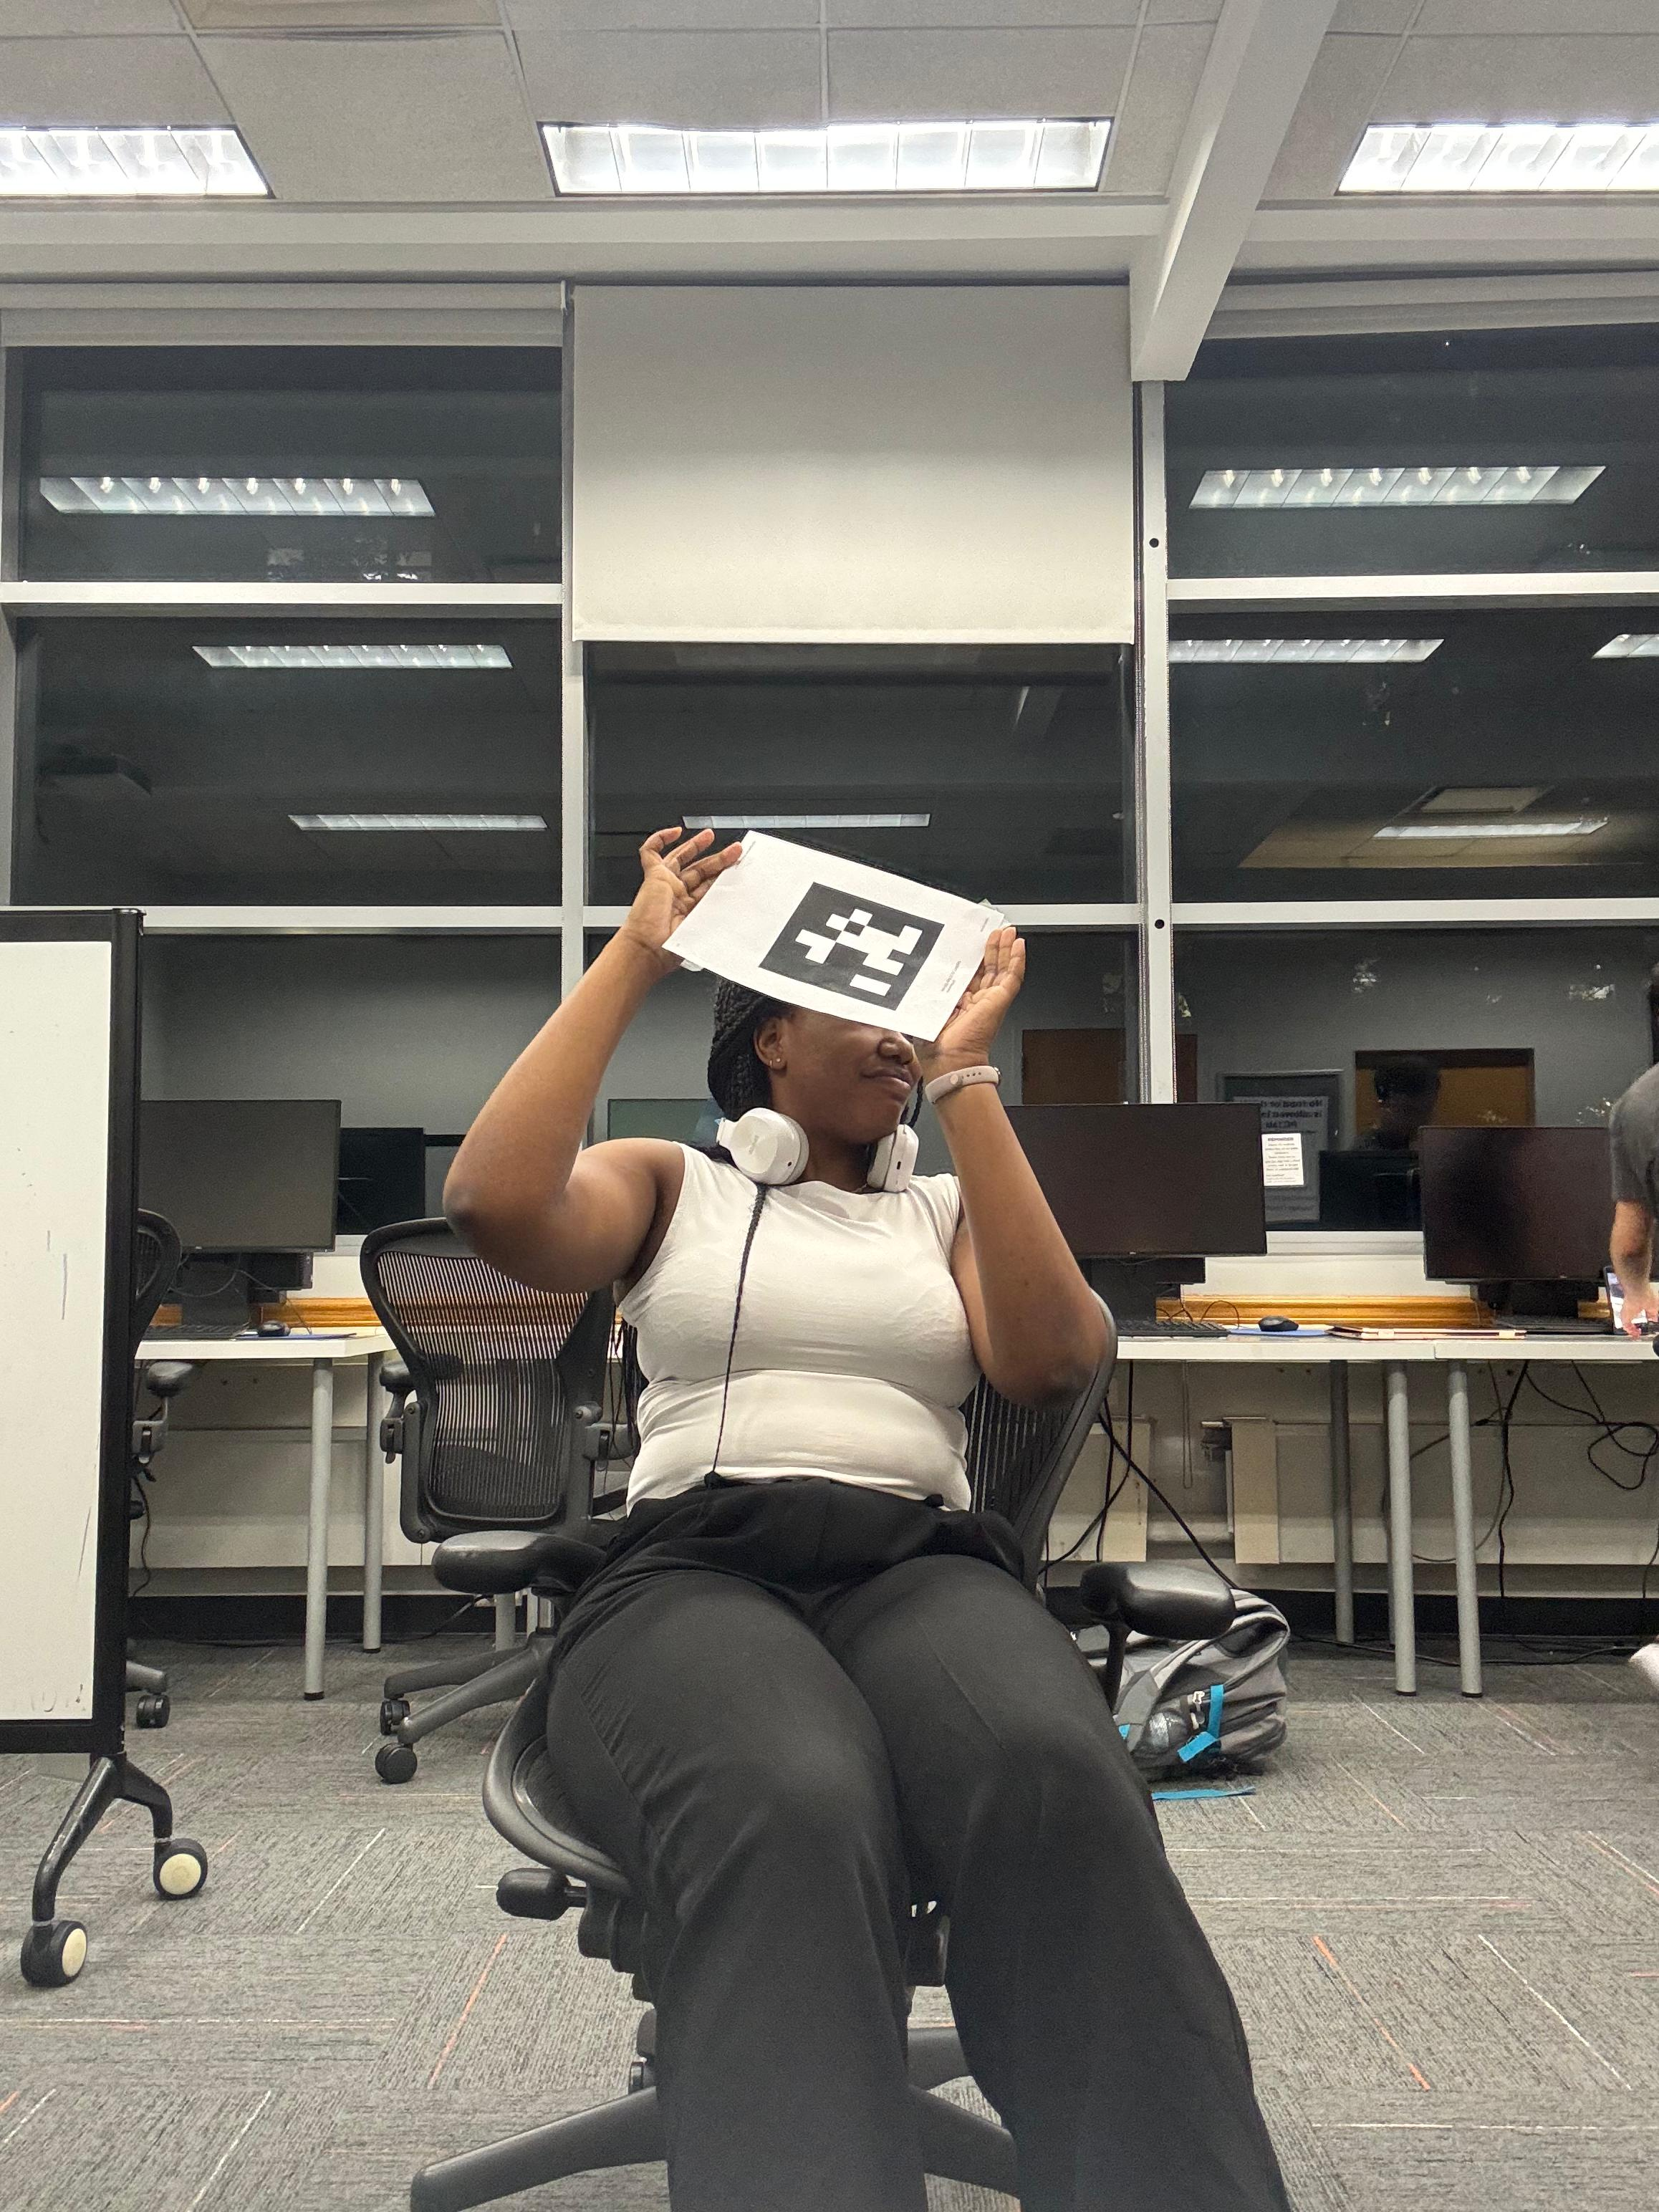
\includegraphics[scale = 0.2]{figs/task4_tag.png}
    \caption{Caption}
    \label{fig:tag before AR}
\end{figure}


\textbf{Tips}: There are many ways to do this, but you may find OpenCV's \texttt{projectPoints}, \texttt{drawContours}, \texttt{addWeighted} and \texttt{line} methods useful. You don't have to use all these methods.

\solution{

\begin{figure}[h!]
    \includegraphics[scale = 0.3]{figs/task4_AR_results.png}

    \label{fig:answer to task 4, me holding an AprilTag}
\end{figure}

}

\end{document}


